%%%%%%%%%%%%%%%%%%%%%%%%%%%%%%%%%%%%%%%%%%%%%%%%%%%%%%%%%%%%%%%%%%%%%%%%%%%%%
% AMEE 2026 E-Poster: Web-Based CCU Orientation Manual
% Reducing Arterial Line-Related Compartment Syndrome Through Digital Education
% Author: Mu-Yang Hsieh MD, PhD, FESC
% Institution: National Taiwan University Hospital Hsinchu Branch
%%%%%%%%%%%%%%%%%%%%%%%%%%%%%%%%%%%%%%%%%%%%%%%%%%%%%%%%%%%%%%%%%%%%%%%%%%%%%

\documentclass[a0paper, portrait, 25pt]{tikzposter}

% Packages
\usepackage[utf8]{inputenc}
\usepackage[T1]{fontenc}
\usepackage{helvet}
\usepackage{graphicx}
\usepackage{multicol}
\usepackage{enumitem}
\usepackage{booktabs}
\usepackage{tikz}
\usetikzlibrary{shapes.geometric, arrows.meta, positioning, calc, shadows, decorations.pathreplacing}
\usepackage{qrcode}
\usepackage{xcolor}
\usepackage{amsmath}
\usepackage{array}
\usepackage{tabularx}
\usepackage{colortbl}

% Color definitions - Professional medical theme
\definecolor{navyblue}{RGB}{26,54,93}
\definecolor{lightnavy}{RGB}{44,82,130}
\definecolor{teal}{RGB}{49,151,149}
\definecolor{lightblue}{RGB}{49,130,206}
\definecolor{coral}{RGB}{229,62,62}
\definecolor{success}{RGB}{56,161,105}
\definecolor{warning}{RGB}{214,158,46}
\definecolor{bglight}{RGB}{241,245,249}
\definecolor{textdark}{RGB}{15,23,42}
\definecolor{textmuted}{RGB}{100,116,139}

% Sans-serif font
\renewcommand{\familydefault}{\sfdefault}

% Custom tikzposter theme
\definecolorstyle{MedicalStyle}{
    \definecolor{colorOne}{named}{navyblue}
    \definecolor{colorTwo}{named}{lightblue}
    \definecolor{colorThree}{named}{teal}
}{
    % Background Colors
    \colorlet{backgroundcolor}{bglight}
    \colorlet{framecolor}{navyblue}
    % Title Colors
    \colorlet{titlebgcolor}{navyblue}
    \colorlet{titlefgcolor}{white}
    % Block Colors
    \colorlet{blocktitlebgcolor}{navyblue}
    \colorlet{blocktitlefgcolor}{white}
    \colorlet{blockbodybgcolor}{white}
    \colorlet{blockbodyfgcolor}{textdark}
    % Innerblock Colors
    \colorlet{innerblocktitlebgcolor}{lightblue}
    \colorlet{innerblocktitlefgcolor}{white}
    \colorlet{innerblockbodybgcolor}{lightblue!10}
    \colorlet{innerblockbodyfgcolor}{textdark}
    % Note colors
    \colorlet{notefgcolor}{textdark}
    \colorlet{notebgcolor}{warning!20}
    \colorlet{noteframecolor}{warning}
}

\usetheme{Default}
\usecolorstyle{MedicalStyle}
\useblockstyle{Default}

% Title formatting
\settitle{
    \centering
    \vbox{
        \centering
        \color{titlefgcolor}
        {\bfseries \Huge \@title \par}
        \vspace*{1em}
        {\Large \@author \par}
        \vspace*{0.5em}
        {\large \@institute \par}
    }
}

% Poster information
\title{\parbox{\linewidth}{\centering Web-Based Interactive CCU Orientation Manual:\\[0.3em] Reducing Arterial Line-Related Compartment Syndrome Through Digital Education}}
\author{Mu-Yang Hsieh MD, PhD, FESC$^{1,2}$, Chen-Wei Lien MD$^{1}$, Ru-Ying Hsu MD$^{1}$, Li-Ta Keng MD$^{1}$}
\institute{$^{1}$Division of Cardiology, National Taiwan University Hospital Hsinchu Branch\\$^{2}$Graduate Institute of Clinical Medicine, National Taiwan University\\[0.5em]\textcolor{lightblue}{\textbf{AMEE 2026 | Glasgow, Scotland | August 22-26, 2026}}}

\begin{document}

\maketitle

\begin{columns}

%----------------------------------------------------------------------
%                     COLUMN 1: BACKGROUND & METHODS
%----------------------------------------------------------------------
\column{0.32}

\block{Background \& Problem}{
    \textbf{\Large The Challenge}\\[0.5em]
    Acute myocardial infarction (AMI) patients in the coronary care unit (CCU) require intensive hemodynamic monitoring. Arterial line placement is a common procedure, but patients on \textbf{dual antiplatelet therapy (DAPT)} combined with \textbf{anticoagulation} face elevated bleeding risks.

    \vspace{1em}
    \innerblock[]{}{
        \textcolor{coral}{\textbf{Critical Issue:}} Brachial artery puncture in anticoagulated patients can lead to \textbf{compartment syndrome}, requiring emergency fasciotomy.
    }

    \vspace{1.5em}
    \textbf{\Large Incidence Data (2022-2025)}

    \vspace{0.5em}
    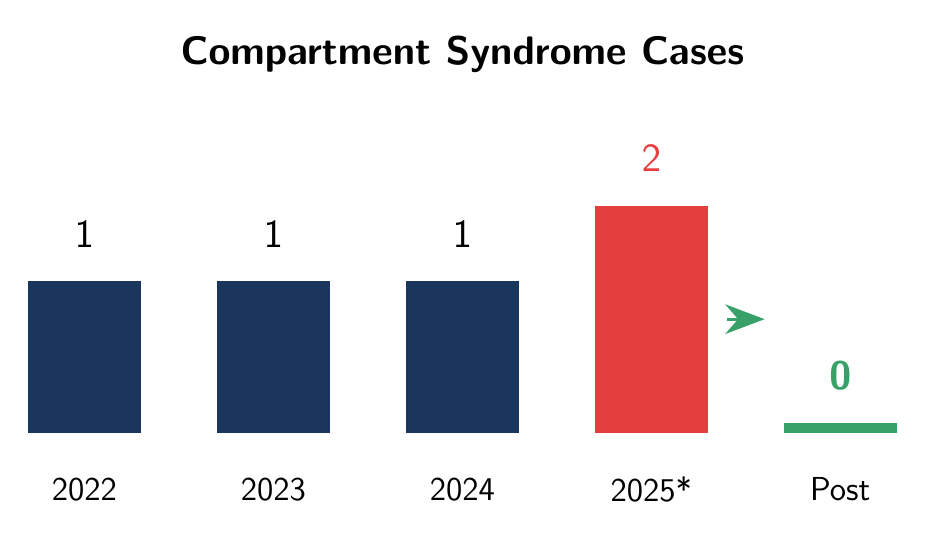
\begin{tikzpicture}[scale=1.2]
        % Bar chart
        \fill[navyblue] (0,0) rectangle (1.2,1.6);
        \fill[navyblue] (2,0) rectangle (3.2,1.6);
        \fill[navyblue] (4,0) rectangle (5.2,1.6);
        \fill[coral] (6,0) rectangle (7.2,2.4);
        \fill[success] (8,0) rectangle (9.2,0.1);

        % Labels
        \node at (0.6,-0.6) {\large 2022};
        \node at (2.6,-0.6) {\large 2023};
        \node at (4.6,-0.6) {\large 2024};
        \node at (6.6,-0.6) {\large 2025*};
        \node at (8.6,-0.6) {\large Post};

        % Values
        \node at (0.6,2.1) {\Large 1};
        \node at (2.6,2.1) {\Large 1};
        \node at (4.6,2.1) {\Large 1};
        \node at (6.6,2.9) {\Large\textcolor{coral}{2}};
        \node at (8.6,0.6) {\Large\textcolor{success}{\textbf{0}}};

        % Title
        \node at (4.6,4) {\Large\textbf{Compartment Syndrome Cases}};

        % Arrow
        \draw[-{Stealth[length=5mm]},very thick,success] (7.4,1.2) -- (7.8,1.2);
    \end{tikzpicture}

    \vspace{0.5em}
    \small *Index case July 2025: 67-year-old male with AMI, multiple brachial artery puncture attempts while on Brilinta + Clexane + Heparin
}

\block{Methods: HFACS Analysis}{
    We applied the \textbf{Human Factors Analysis and Classification System (HFACS)} framework to identify root causes and design educational interventions.

    \vspace{1em}
    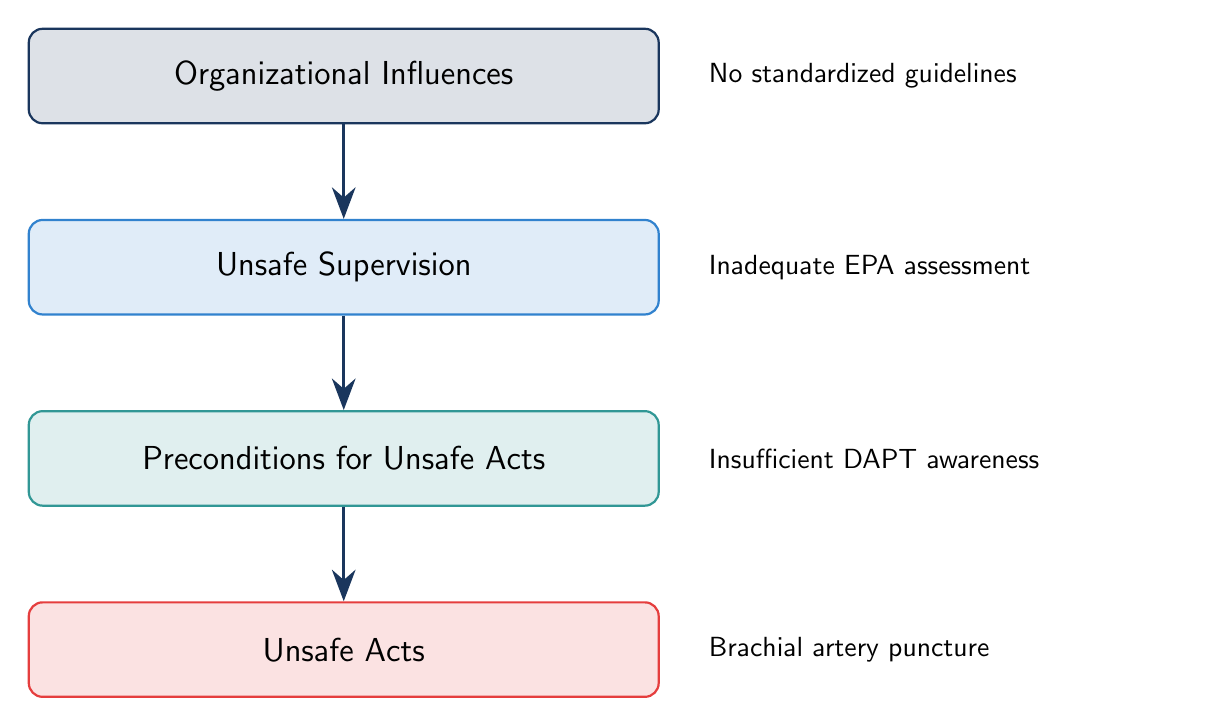
\begin{tikzpicture}[
        node distance=1.2cm,
        box/.style={rectangle, draw=#1, fill=#1!15, thick, minimum width=8cm, minimum height=1.2cm, text centered, rounded corners=5pt, font=\large},
        arrow/.style={-{Stealth[length=4mm]}, very thick, navyblue}
    ]
        % HFACS Levels
        \node[box=navyblue] (org) {Organizational Influences};
        \node[box=lightblue, below=of org] (sup) {Unsafe Supervision};
        \node[box=teal, below=of sup] (pre) {Preconditions for Unsafe Acts};
        \node[box=coral, below=of pre] (act) {Unsafe Acts};

        % Arrows
        \draw[arrow] (org) -- (sup);
        \draw[arrow] (sup) -- (pre);
        \draw[arrow] (pre) -- (act);

        % Side labels
        \node[right=0.5cm of org, text width=6cm, font=\normalsize, align=left] {No standardized guidelines};
        \node[right=0.5cm of sup, text width=6cm, font=\normalsize, align=left] {Inadequate EPA assessment};
        \node[right=0.5cm of pre, text width=6cm, font=\normalsize, align=left] {Insufficient DAPT awareness};
        \node[right=0.5cm of act, text width=6cm, font=\normalsize, align=left] {Brachial artery puncture};
    \end{tikzpicture}

    \vspace{1em}
    \innerblock[]{Root Causes Identified}{
        \begin{enumerate}[leftmargin=2em, itemsep=0.3em]
            \item Lack of standardized arterial line placement guidelines
            \item No risk stratification for anticoagulated patients
            \item Insufficient education on DAPT bleeding complications
            \item Missing EPA-based competency assessment
        \end{enumerate}
    }
}

\block{Study Design}{
    \textbf{Intervention Period:} August 2025 -- Present\\
    \textbf{Setting:} 10-bed CCU, tertiary medical center\\
    \textbf{Target Learners:} Residents, Nurse Practitioners\\[0.5em]

    \textbf{Educational Framework:}
    \begin{itemize}[leftmargin=2em, itemsep=0.4em]
        \item Root Cause Analysis-driven curriculum
        \item Competency-Based Medical Education (CBME)
        \item Entrustable Professional Activities (EPA)
        \item Just-in-time digital learning resources
    \end{itemize}
}

%----------------------------------------------------------------------
%                     COLUMN 2: THE INTERVENTION
%----------------------------------------------------------------------
\column{0.36}

\block{The Intervention: Interactive Web-Based Manual}{
    \begin{center}
        {\bfseries \LARGE CCU Orientation Manual v2.1}\\[0.3em]
        \large React-based Single-Page Application
    \end{center}

    \vspace{1em}

    \innerblock[]{9 Interactive Modules}{
        \begin{multicols}{2}
        \begin{enumerate}[leftmargin=2em, itemsep=0.2em, font=\large]
            \item Daily Checklist
            \item Safety Cases
            \item ACS Orders
            \item HF Certification
            \item Special Care
            \item Drug Reference
            \item Emergency Protocols
            \item Chart Writing Guide
            \item Self-Assessment Quiz
        \end{enumerate}
        \end{multicols}
    }

    \vspace{1.5em}
    {\bfseries \Large Key Educational Features:}

    \vspace{1em}
    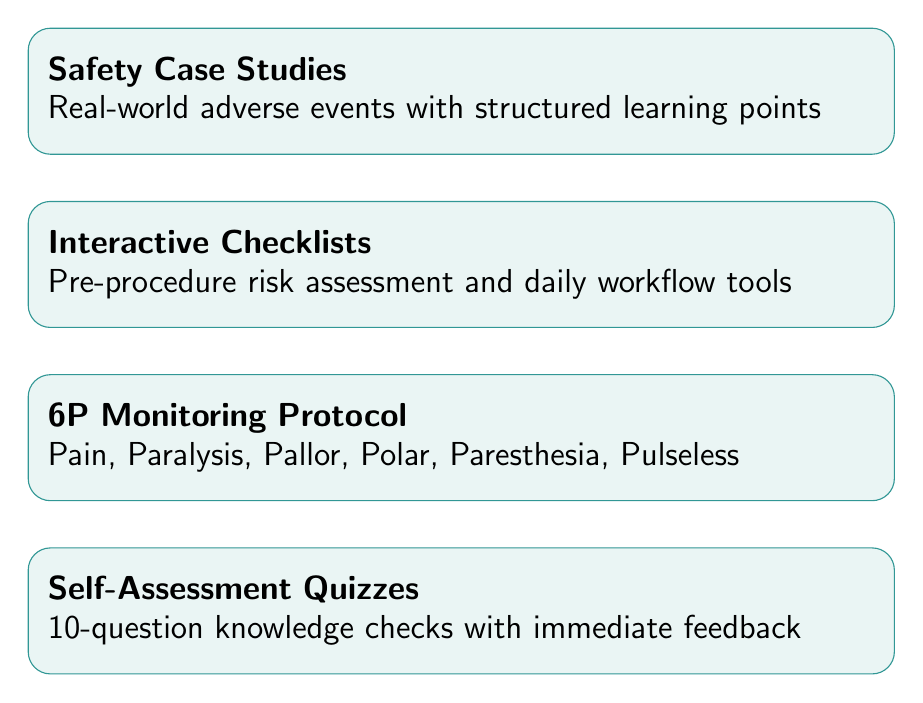
\begin{tikzpicture}[
        feature/.style={rectangle, draw=teal, fill=teal!10, rounded corners=8pt, minimum width=11cm, minimum height=1.6cm, text width=10.5cm, align=left, font=\large}
    ]
        \node[feature] at (0,0) {\textbf{Safety Case Studies}\\Real-world adverse events with structured learning points};
        \node[feature] at (0,-2.2) {\textbf{Interactive Checklists}\\Pre-procedure risk assessment and daily workflow tools};
        \node[feature] at (0,-4.4) {\textbf{6P Monitoring Protocol}\\Pain, Paralysis, Pallor, Polar, Paresthesia, Pulseless};
        \node[feature] at (0,-6.6) {\textbf{Self-Assessment Quizzes}\\10-question knowledge checks with immediate feedback};
    \end{tikzpicture}

    \vspace{2em}
    \innerblock[]{}{
        \centering
        \textcolor{coral}{\textbf{\Large Critical Safety Message Embedded:}}\\[0.5em]
        \large ``If patient is on Brilinta/Prasugrel + anticoagulation,\\
        \textbf{DO NOT} perform brachial artery puncture''
    }

    \vspace{2em}
    \begin{center}
        {\bfseries \Large Scan to Access the Manual:}\\[1em]
        \qrcode[height=5cm]{https://ntuh-hsinchu-cv.github.io/ccu-orientation-manual.html}\\[0.5em]
        \large\texttt{ntuh-hsinchu-cv.github.io/ccu-orientation-manual.html}
    \end{center}
}

\block{Arterial Line Placement Algorithm}{
    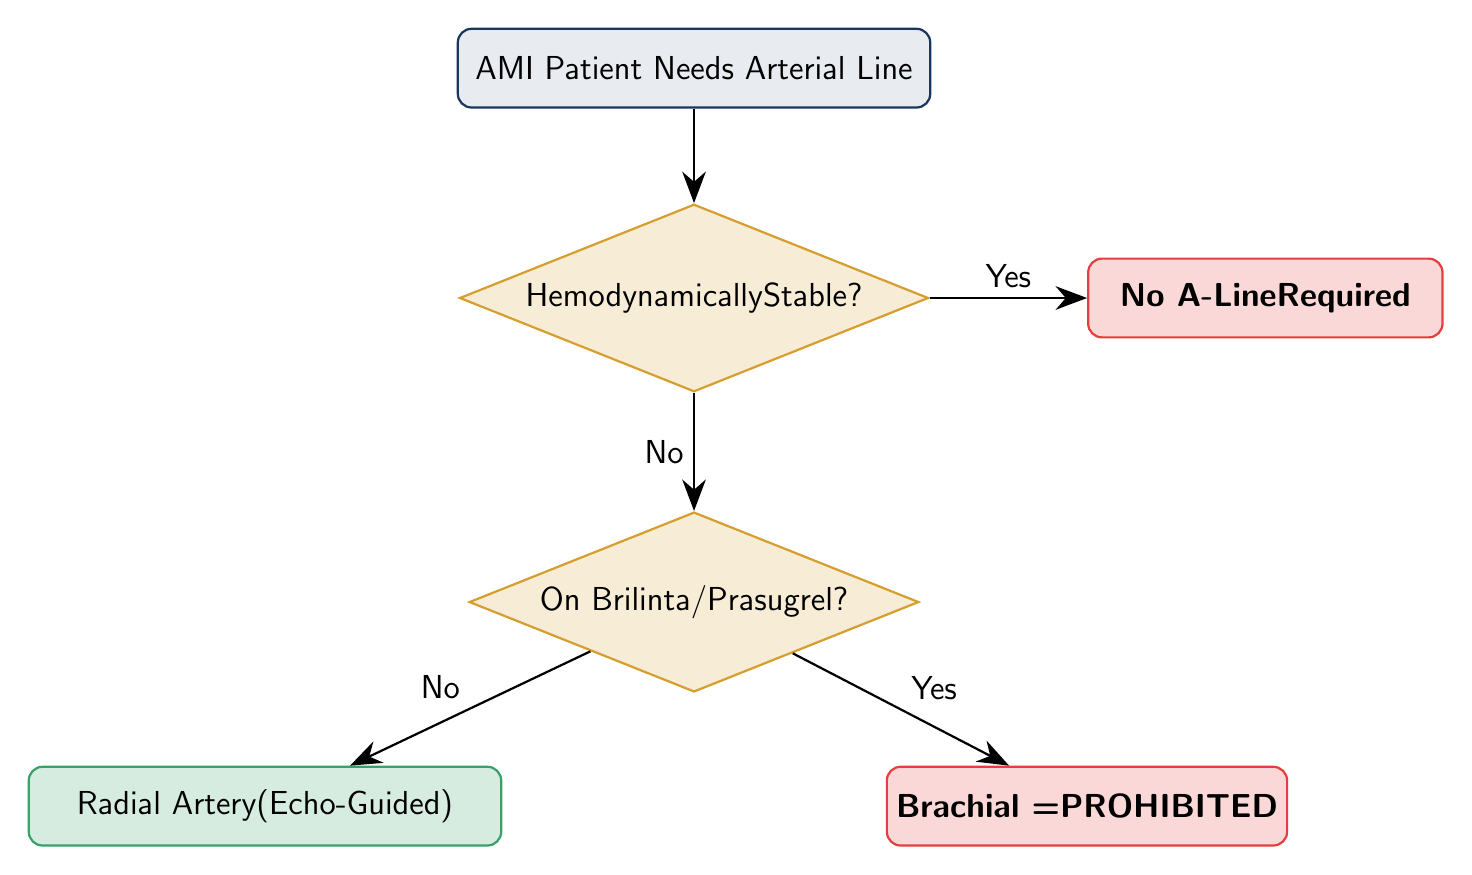
\begin{tikzpicture}[
        node distance=1cm,
        decision/.style={diamond, draw=warning, fill=warning!20, thick, aspect=2.5, inner sep=3pt, font=\large},
        process/.style={rectangle, draw=navyblue, fill=navyblue!10, rounded corners=5pt, thick, minimum width=6cm, minimum height=1cm, font=\large, text centered},
        stop/.style={rectangle, draw=coral, fill=coral!20, rounded corners=5pt, thick, minimum width=4.5cm, minimum height=1cm, font=\large\bfseries, text centered},
        go/.style={rectangle, draw=success, fill=success!20, rounded corners=5pt, thick, minimum width=6cm, minimum height=1cm, font=\large, text centered},
        arrow/.style={-{Stealth[length=4mm]}, thick}
    ]
        \node[process] (start) {AMI Patient Needs Arterial Line};
        \node[decision, below=1.2cm of start] (stable) {Hemodynamically\\Stable?};
        \node[stop, right=2cm of stable] (no) {No A-Line\\Required};
        \node[decision, below=1.5cm of stable] (dapt) {On Brilinta/\\Prasugrel?};
        \node[go, below left=1.5cm and 1cm of dapt] (radial) {Radial Artery\\(Echo-Guided)};
        \node[stop, below right=1.5cm and 1cm of dapt] (nobrachial) {Brachial =\\PROHIBITED};

        \draw[arrow] (start) -- (stable);
        \draw[arrow] (stable) -- node[above]{\large Yes} (no);
        \draw[arrow] (stable) -- node[left]{\large No} (dapt);
        \draw[arrow] (dapt) -- node[above left]{\large No} (radial);
        \draw[arrow] (dapt) -- node[above right]{\large Yes} (nobrachial);
    \end{tikzpicture}

    \vspace{0.5em}
    \textbf{Post-removal monitoring:} 6P assessment every 15 minutes for 1 hour before ICU discharge
}

%----------------------------------------------------------------------
%                     COLUMN 3: RESULTS & CONCLUSIONS
%----------------------------------------------------------------------
\column{0.32}

\block{Results}{
    {\bfseries \Large Primary Outcome}

    \vspace{1em}
    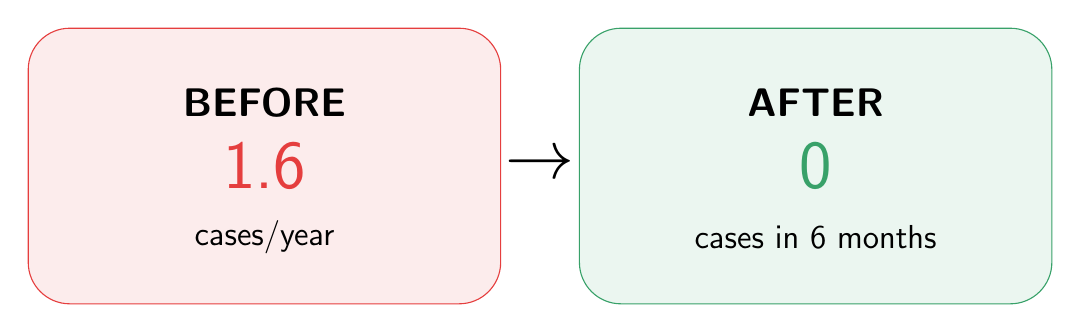
\begin{tikzpicture}
        % Before box
        \node[rectangle, draw=coral, fill=coral!10, rounded corners=15pt, minimum width=6cm, minimum height=3.5cm] at (0,0) {};
        \node at (0,0.8) {\Large\textbf{BEFORE}};
        \node at (0,0) {\textcolor{coral}{\fontsize{60}{72}\selectfont 1.6}};
        \node at (0,-0.9) {\large cases/year};

        % Arrow
        \node at (3.5,0) {\fontsize{48}{60}\selectfont $\rightarrow$};

        % After box
        \node[rectangle, draw=success, fill=success!10, rounded corners=15pt, minimum width=6cm, minimum height=3.5cm] at (7,0) {};
        \node at (7,0.8) {\Large\textbf{AFTER}};
        \node at (7,0) {\textcolor{success}{\fontsize{60}{72}\selectfont 0}};
        \node at (7,-0.9) {\large cases in 6 months};
    \end{tikzpicture}

    \vspace{1em}
    \innerblock[]{}{
        \centering
        \textbf{\textcolor{success}{\LARGE 100\% Reduction}} \\in arterial line-related compartment syndrome incidents
    }

    \vspace{1.5em}
    {\bfseries \Large Secondary Outcomes}

    \begin{center}
    \renewcommand{\arraystretch}{1.6}
    \begin{tabular}{>{\raggedright\arraybackslash}p{7cm} c c}
        \toprule
        \textbf{\large Metric} & \textbf{\large Before} & \textbf{\large After} \\
        \midrule
        Radial artery first-choice rate & 65\% & \textcolor{success}{\textbf{95\%}} \\
        Echo-guided puncture rate & 40\% & \textcolor{success}{\textbf{90\%}} \\
        6P monitoring compliance & --- & \textcolor{success}{\textbf{100\%}} \\
        Quiz pass rate ($\geq$80\%) & --- & \textcolor{success}{\textbf{92\%}} \\
        \bottomrule
    \end{tabular}
    \end{center}

    \vspace{1.5em}
    {\bfseries \Large Implementation Timeline}

    \vspace{0.5em}
    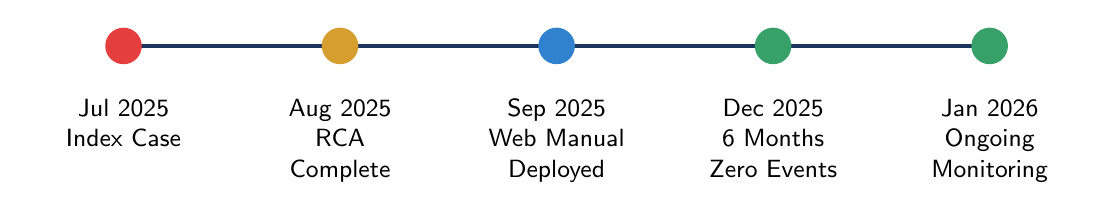
\begin{tikzpicture}[scale=1.1]
        % Timeline
        \draw[very thick, navyblue] (0,0) -- (10,0);

        % Events
        \fill[coral] (0,0) circle (6pt);
        \fill[warning] (2.5,0) circle (6pt);
        \fill[lightblue] (5,0) circle (6pt);
        \fill[success] (7.5,0) circle (6pt);
        \fill[success] (10,0) circle (6pt);

        % Labels
        \node[below, text width=2.2cm, align=center, font=\small] at (0,-0.5) {Jul 2025\\Index Case};
        \node[below, text width=2.2cm, align=center, font=\small] at (2.5,-0.5) {Aug 2025\\RCA\\Complete};
        \node[below, text width=2.2cm, align=center, font=\small] at (5,-0.5) {Sep 2025\\Web Manual\\Deployed};
        \node[below, text width=2.2cm, align=center, font=\small] at (7.5,-0.5) {Dec 2025\\6 Months\\Zero Events};
        \node[below, text width=2.2cm, align=center, font=\small] at (10,-0.5) {Jan 2026\\Ongoing\\Monitoring};
    \end{tikzpicture}
}

\block{Discussion}{
    \textbf{\large Why Web-Based Education Works:}
    \begin{itemize}[leftmargin=2em, itemsep=0.4em]
        \item \textbf{Accessibility:} 24/7 mobile-friendly access
        \item \textbf{Interactivity:} Active learning with quizzes
        \item \textbf{Just-in-time:} Available at point of care
        \item \textbf{Updateable:} Rapid iteration based on new cases
    \end{itemize}

    \vspace{1em}
    \textbf{\large Integration with CBME Framework:}
    \begin{itemize}[leftmargin=2em, itemsep=0.4em]
        \item EPA-based competency milestones
        \item Formative assessment via self-quizzes
        \item Workplace-based learning resources
    \end{itemize}

    \vspace{1em}
    \textbf{\large Limitations:}
    \begin{itemize}[leftmargin=2em, itemsep=0.4em]
        \item Single-center study
        \item Short follow-up period (6 months)
        \item Multiple concurrent interventions
    \end{itemize}
}

\block{Conclusions \& Take-Home Messages}{
    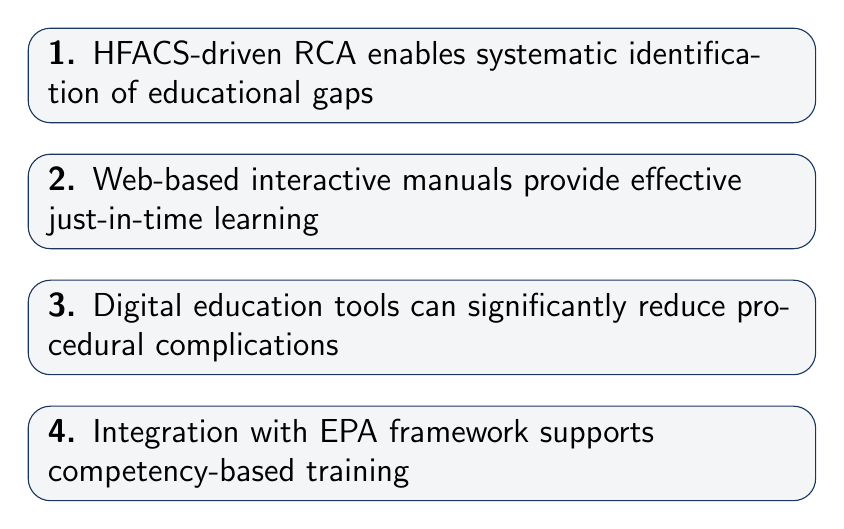
\begin{tikzpicture}[
        msg/.style={rectangle, draw=navyblue, fill=navyblue!5, rounded corners=8pt, minimum width=10cm, minimum height=1.2cm, font=\large, text width=9.5cm, align=left}
    ]
        \node[msg] at (0,0) {\textbf{1.} HFACS-driven RCA enables systematic identification of educational gaps};
        \node[msg] at (0,-1.6) {\textbf{2.} Web-based interactive manuals provide effective just-in-time learning};
        \node[msg] at (0,-3.2) {\textbf{3.} Digital education tools can significantly reduce procedural complications};
        \node[msg] at (0,-4.8) {\textbf{4.} Integration with EPA framework supports competency-based training};
    \end{tikzpicture}

    \vspace{1em}
    \innerblock[]{Future Directions}{
        \centering
        Multi-center implementation $\bullet$ Long-term outcome tracking $\bullet$ AI-powered adaptive learning modules
    }
}

\block{References \& Contact}{
    \small
    \textbf{References:}
    \begin{enumerate}[leftmargin=2em, itemsep=0.2em]
        \item Wiegmann DA, Shappell SA. HFACS Analysis of Military and Civilian Aviation Accidents. \textit{Aviat Space Environ Med}. 2001.
        \item Ten Cate O. Entrustability of professional activities and competency-based training. \textit{Med Educ}. 2005.
        \item Frank JR, et al. Competency-based medical education: theory to practice. \textit{Med Teach}. 2010.
    \end{enumerate}

    \vspace{0.5em}
    \textbf{Acknowledgments:} CCU Nursing Staff, Quality Improvement Committee, NTUH Hsinchu Branch\\
    \textbf{Disclosures:} None\\
    \textbf{Contact:} \texttt{muhsieh@ntuh.gov.tw}
}

\end{columns}

\end{document}
